\section{Scrum}\label{sec:scrum}
Scrum er et framework til at udarbejde og vedligeholde komplekse produkter og løbende levere 
værdi til en kunde gennem inkrementelle og iterative processer/teknikker. 
Dette agile framework har været hyppigt anvendt til softwareudvikling siden 1990’erne. 
Frameworket anses for at være let forståeligt, simpelt sammensat, men svært at mestre.

\subsection{Roller}
I Scrum er de fleste interessenter inddelt i roller. Disse roller er ikke nødvendigvis definitive. Det vil sige at
en person godt kan skifte rolle undervejs i udviklingsforløbet. Nedenfor vil rollerne blive beskrevet.

\subsubsection{Product Owner}
De primære ansvarsområder en Product Owner påtager sig, er at sikre teamet leverer så 
meget værdi til kunden som muligt. Dette sikres gennem vedligeholdelse af Product Backlog’en. 
Den forretning eller virksomhed, som har bestilt et produkt bliver repræsenteret gennem 
Product Owner, som i den forbindelse sikre at teamet arbejder på at levere det funktionalitet, 
som er vigtigst for kunden. Kort fortalt er stakeholders, releases og backlog hovedområderne for en Product Owner.

\subsubsection{Scrum Master}    
Scrum masteren hjælper til med at udføre de artifakter der er i projektet, sikrer at der holdes gode demoer, 
gode retrospectives og sikrer at Product Owner’en groomer backloggen. Product Owner’en holdes i snor med alle Scrum processer blandt andet 
klargøring af næste sprint, prioriteter og om noget skal skiftes ud eller erstattes i backloggen.\\

Nedenfor listes Scrum Masterens funktioner og ansvarsområder:

\begin{itemize}
    \item Ejer processerne i Scrum og deres eksekvering.
    \item Faciliterer de forskellige events.
    \item Er ikke en chef eller autoritet.
    \item Sikrer at Product Owner’en arbejder med teamet, for at få sprintet og releases til at fungere.
    \item Estimeringer kommer i god tid løbende i et sprint, så man er klar til næste planning.
    \item Sørger for at ingen forstyrer teamet og der er et roligt og trygt miljø omkring udviklings teamet.
    \item Sikrer at backloggen bliver groomet i løbet af sprintet.
    \item Sikrer at Product Owner’en er i løbende kontakt med stakeholders og kunden, for at sikre maksimal værdi.
    \item Sikrer at Product Owner’en, i samarbejde med kunden og stakeholders, har udvalgt nok stories til at dække næste sprint og gerne lidt flere.
\end{itemize}


\subsubsection{Dev Team}
Udviklingsteamet er de mennesker som normalt udarbejder selve produktet, altså udviklere, designere 
eller ingeniører osv. Teamet arbejder som en enhed, og regulerer selv sine opgaver og udviklingsmetoder. 
Her handler det om, at alle hjælper alle med at opnå de fælles mål for et givet sprint. Det vil sige 
at teamet har mulighed for at træffe egne valg og ikke behøver indrage hverken Scrum Master’en eller 
Product Owner’en i beslutningen, når det har noget med udvikling af gøre.

\subsection{Artefakter}
I sidste semester beskæftigede gruppen sig med UP, som indeholder en lang række artefakter. I scrum findes en mindre mængde af 
artefakter, og nedenfor vil disse blive beskrevet.

\subsubsection{Product Backlog}
En product backlog en liste af user stories I ordnet rækkefølge efter, hvilken værdi det bringer kunden. 
Det er den eneste liste af krav til et givet projekt. Denne liste vedligeholdes og udarbejdes af 
Product Owner’en. En backlog er ikke en låst liste, men en liste der hele tiden kan ændre sig, og få 
tilføjet eller fjernet nye elementer, alt efter hvad der bringer kunden værdi. 

\subsubsection{Sprint Backlog}
En sprint backlog er en anden liste som indeholder de stories og tasks som er udvalgt til et givet sprint. Denne indeholder ydermere målene for sprintet. 

\subsubsection{Burndown chart}
Et burndown chart er en graf der helt simpelt viser, om udviklingsteamet er foran eller bagefter tidsplanen. Et burndown chart er baseret på hvor mange timer 
teamet har til rådighed i et sprint, og indeholder to grafer. Den ene graf viser hvor mange timer teamet har tilbage efter hver arbejdsdag, hvis alt går som planlagt.
Den anden graf viser hvor langt tid teamet selv estimerer at de har tilbage. Et burndown chart viser altså ikke hvor meget tid udviklerne har brugt, men derimod hvor meget
tid de har tilbage, baseret på estimationer.

\subsection{Ceremonier}
Scrum frameworket består af en række ceremonier. Disse vil kort blive beskrevet nedenfor.

\subsubsection{Sprint}
Et sprint er en tidsperiode hvori et potentielt “færdigt” og produktionsklart product increment bliver udarbejdet. 
Et increment er en sum af alle de udvalgte user stories fra backlog'en. Et sprint vil normalt vare mellem 1 og 4 uger 
afhængig af projektets størrelse og firmaets ressourcer.

\subsubsection{Sprint planning}
Sprint planning er et “møde” hvori gruppen/teamet udarbejder en plan for det kommende sprint. Dette møde må ikke vare mere end 8 timer. 
Her giver Dev Team'et sit forslag til hvilke eller hvor mange stories de kan nå at udarbejde, beregnet ud fra deres velocity 
og med fokus på hvor meget de nåede i sidste sprint.

\subsubsection{Daily standup meeting}
Et daily standup meeting er et lille “møde” hvor teamet er samlet og besvarer 3 spørgsmål. Første spørgsmål er “Hvad gjorde folk i går” 
altså hvad arbejder de på. Det næste er “Hvad vil du lave i dag?” Hvilket giver teamet mulighed for at få en fælles 
forståelse for hvad alle laver. Til sidst “Er der noget som forhindrer dig i at udføre dit arbejde i dag?”. 
Det kunne være viden, redskaber eller andet som et medlem mangler for at gøre sit arbejde.

\subsubsection{Sprint review}
Et sprint review er en “demo” visning af selve systemet for hele teamet samt så mange udefrakommende som muligt. Ofte er kunden også til stede ved dette review.

\subsubsection{Sprint retrospective}
Denne ceremoni handler om indsigt, forbedring og hvordan det sidste sprint har forløbet sig. Her udarbejdes et kort dokument, som kan bruges til næste sprint planning.

\section{Extreme Programming}\label{sec:xp}
Extreme Programming (XP) er en agil udviklingsmetode, brugt til at fremstille software. Metoden byder på 15 regler som skal følges. XP handler om at arbejde i det ekstreme, 
hvis noget virker skal man gøre til dets ekstreme mulighed.  \\

XP har 5 kerneværdier; Respect, Communication, Simplicity, Feedback og Courage. Hertil 12 praktikker som 
skal følges og efterleves til ekstrem hvis metoden skal anvendes korrekt. \\

Scrum er som beskrevet tidligere i afsnittet et framework til udvikling af produkter, ofte software løsninger, 
hvilket fungerer som en container for mange virksomheder, hvor andre praktikker kan tilføjes til. XP er i den 
forbindelse en af de praktikker som ofte tilføjes til Scrum, ihvertfald nogle af dets regler. \\

Nogle af XP’s regler er svære at overholde og reglerne anses for at være uden undtagelse, altså alle regler 
og praktikker skal anvendes til det ekstreme. Derimod er nogle af XP’s praktikker en god supplering til 
Scrum frameworket og det kan hjælpe et nyt, eller uerfarent team til at udvikle sig indenfor det agile 
univers og Scrum frameworket. \\

Det kan endvidere udledes at XP og agil udvikling er lidt paradoksalt fordi et team har et mål om at være helt selv organiserende men får 
samtidigt at vide at de “skal” have en bestemt længde arbejdsuge, programmere sammen 2 og 2 og implementere “Test Driven Development”. 

\section{Kanban}\label{sec:kanban}
Denne udviklingsmetode er bygget på at visualisere og skabe flow i arbejdet for det givne team. Kanban giver 
mulighed for hurtigt at genprioritere arbejdsopgaver og omstillingspararthed i forbindelse med pludselige ændringer. 
Kanban er en esktrem agil udviklingsmetode, som har færre "regler".\\

Kanban\cite{Kanban} bruger i modsætning til Scrum, ikke sprints. Teamet arbejder i et langt kontinuerligt flow, hvor der releases
når teamet føler de har færdiggjort noget brugbart software. Hvis teamet har brug for at lave nogle ændringer,
venter de ikke til næste sprint, ligesom i Scrum, men ændrer det med det samme. \\

Kanban gør sig speciel ved at have en begrænsning, på hvor meget arbejde der kan være "in-progress" på én gang. 
Dette sikrer at udviklerteamet færdiggører de påbegyndte opgaver, inden der startes på noget nyt. 
I gennem visualiseringen bliver det derfor også nemt for kunden at se hvor langt teamet er kommet og
hvad der arbejdes på.\\

\textbf{Kanban i Scrum}\\
Kanban bruges i Scrum med "limited work in progeess", for at sikre at der ikke arbejdes på for meget på én gang.
I sprints anvendes det, for at undgå halvfærdige opgaver til slut i sprintet, eller at teamet pludselig skal løbe stærkt.
Hermed sikres det at kunne fremvise en demo, ved slutningen af sprintet i review'et.\\

Der er højest 1 eller 2 stories igang, afhængig af teamets størrelse, på samme tid. Det er et krav at teamet færdiggører opgaver 
inden nogen påtager sig nye opgaver. Product owneren har ansvar for, at teamet færdiggører påbegyndte opgaver i sprintet. 

\section{Metodevalg}\label{sec:valgafvaektoej}
Gruppen har valgt at benytte Scrum til dette projekt. Dette er gjort fordi Scrum ligger et godt fundament 
for software-udvikling generelt. Kundens krav til systemet er ikke altid forudbestemt, og kan ændres hele tiden. 
Her er det vigtigt at kunne være fleksibel, og have en agil tankegang. \\

Extreme Programming er også blevet brugt til en vis grad. Gruppen har valgt at implementere nogle få 
af de 12 praktikker som findes i XP. 
\begin{enumerate}
    \item Pair Programming
    \begin{itemize}
        \item Har sikret enighed om hvordan koden skal laves, og sikret en højere kvalitet af arbejdet.
    \end{itemize}

    \item Code Refactoring
    \begin{itemize}
        \item Har sørget for at koden har opretholdt en vis standard, og i så høj grad som muligt sørget for ”Low coupling \& High Cohesion”
    \end{itemize}
    
    \item Collective Code Ownership
    \begin{itemize}
        \item Alle medlemmer af gruppen ejer koden. Det har været muligt at gennemse og opdatere hinandens kode. 
        Brugen af Git har hjulpet med dette. 
    \end{itemize}
\end{enumerate}

Mere om XP praktikker i kapitel \ref{ch:kvalitetssikring}\\

Det kan være svært for en gruppe studerende, at designe et software-system ned til mindste detalje, 
tage højde for hver eneste metode, og kortlægge hver enkelte klasse i systemet, inden man begynder at kode. 
Derfor er det godt at kunne benytte en agil udviklingsmetode, hvor det er muligt for gruppen at ændre kurs og 
lave nogle ændringer til krav og kode løbende. \\

En måde hvorpå et team kan finde den rette udviklingsmodel, er vha. et Boehm-Chart, som kan ses i Figur \ref{fig:Boehm}. 
Denne model gør det muligt at fastlægge hvor agil en gruppe er, og omvendt. \\

\begin{figure}[H]
    \centering
    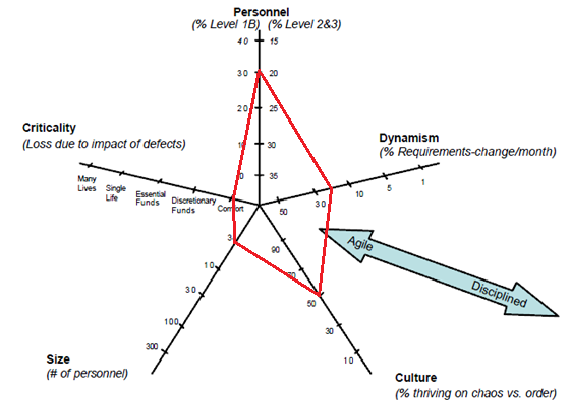
\includegraphics[width=0.7\textwidth]{figures/Boehm-chart.png}
    \caption{Boehm-Chart}
    \label{fig:Boehm}
\end{figure}

Et Boehm-Chart består af 5 forskellige parametre, hvor der tegnes en streg fra hver gren til den næste. 
Jo tættere resultatet er på midten, desto mere agil er teamet. 
For gruppens projekt, trækker størrelsen af gruppen og alvorligheden af problemstilling i den agile retning. 
Et biograf bookings system er ikke en kritisk problemstilling. \\

Derimod hvis projektet har med menneskeliv at gøre, 
bliver alvorligheden selvfølgelig høj, og det er derfor vigtigt at planlægge et hvert scenarie, 
hvilket er lig en plandreven udviklingsmetode.
Hvis man ser på figuren, ville en agil-udviklingsmodel såsom Scrum passe fint til teamet og projektet. 
